\documentclass{beamer}

\usetheme{metropolis}           % Use metropolis theme
\usefonttheme[onlymath]{serif}

\usepackage{xeCJK}
\usepackage{graphicx}
\usepackage{amsmath}
\usepackage{multicol}
\usepackage[font=small,labelfont=bf]{caption}
\DeclareCaptionFont{mysize}{\fontsize{7}{9.6}\selectfont}
\captionsetup{font=mysize}

\title{工作总结}
\date{\today}
\author{林连升}
%\institute{福州大学 数学与计算机科学学院}

\begin{document}
  \maketitle

  \begin{frame}{一些微小的工作}
    \begin{itemize}
    \item \textbf{Word Similarity at NLPCC-2016} \newline
    \item \textbf{DBQA at NLPCC-2017} \newline
      Document-Based Question Answering
    \item \textbf{STC-2 at NTCIR-13} \\
      Short Text Conversation
    \end{itemize}
    \end{frame}
  \section{Word Similarity}

    \begin{frame}{数据集: PKU-500}
    \begin{center}
      \begin{figure}
      \includegraphics[width=4in,height=2.2in]{pku-500-1.jpg}
      %\caption{}
      \end{figure}
      \end{center}
    \end{frame}

    \begin{frame}{数据集: PKU-500}
    \begin{center}
      \begin{figure}
      \includegraphics[width=4in,height=2.5in]{pku-500-2.jpg}
      %\caption{}
      \end{figure}
      \end{center}
    \end{frame}

    \begin{frame}{评测指标}
     Spearman's rank correlation coefficient: 
     \begin{equation}
        p = 1 - \frac{6\sum_{i=1}^n{(R_{Xi} - R_{Yi})^2}}{n(n^2 - 1)}
     \end{equation}
     where n is the number of word pairs being evaluated, $R_{Xi}$ and $R_{Yi}$ 
     are the standard deviations of the rank of automatic computing results and 
     human labelled scores, respectively.
    \end{frame}

    \begin{frame}{评测结果}
    \begin{center}
      \begin{figure}
      \includegraphics[width=4in,height=2.8in]{ws-result.png}
      %\caption{}
      \end{figure}
      \end{center}
    \end{frame}

    \begin{frame}{我的结果}
      \begin{itemize}
      \item Word2Vec + 同义词词林 + 知网 \\
      Spearman value = 0.58
      \end{itemize}
    \end{frame}

    \begin{frame}{Word2Vec}
    \begin{itemize}
      \item 2G 新闻语料 (12对词未覆盖)\\
      Spearman value = 0.338
      \item 2G 新闻语料 + 补充语料 \\
      Spearman value = 0.400
    \end{itemize}
    \end{frame}

    \begin{frame}{同义词词林}
    参考三篇Paper: 
    \begin{itemize}
      \item [1]田久乐,赵蔚. 基于同义词词林的词语相似度计算方法[J]. 吉林大学学报(信息科学版),2010,06:602-608. \\
      \item [2]吕立辉,梁维薇,冉蜀阳. 基于词林的词语相似度的度量[J]. 现代计算机(专业版),2013,01:3-6+9. \\
      \item [3]朱新华,马润聪,孙柳,陈宏朝. 基于知网与词林的词语语义相似度计算[J]. 中文信息学报,2016,04:29-36. \\
    \end{itemize}
    \end{frame}

    \begin{frame}{同义词词林简介}
    \begin{center}
      \begin{figure}
      \includegraphics[width=3.1in,height=1.5in]{cilin1.png}
      %\caption{}
      \end{figure}
      \begin{figure}
      \includegraphics[width=4.1in,height=1.2in]{cilin2.png}
      %\caption{}
      \end{figure}
      \end{center}
    \end{frame}

    \begin{frame}{田久乐等的算法,2010}
    \begin{center}
      \begin{itemize}
        \item 主要思想:基于同义词词林的结构, 利用词语中义项的编号, 根据两个义项的语义距离, 计算出义项相似度。\\
        \item 首先判断在同义词林中作为叶子节点的两个义项在哪一层开始分支。例如: Aa01A01与 Aa01B01, 即在第4层分支。在每一层分支,分别对应一个系数,然后再乘以调节参数。\\
      \end{itemize}
    \end{center}
    \end{frame}

    \begin{frame}{田久乐等的算法,2010}
    \begin{center}
      \begin{figure}
      \includegraphics[width=3.9in,height=2in]{cilin-method-2010.png}
      \caption{这里n是分支数,k是两个分支的距离,abcdf是实验得到的系数。}
      \end{figure}
      \end{center}
    \end{frame}

    \begin{frame}{田久乐等的算法,2010}
    举个例子: \\
    Ae05A01= 邮递员 \ 邮差 \ 信差 \ 信使 \ 绿衣使者 \ 通信员 \ 投递员 \\
    Ae05A02= 交通员 \ 交通 \ 通讯员 \\
    Ae05A03= 联络员 \ 联络官 \ 联系人 \\
    其中,义项“邮递员”和“联络员”在第五层分支,分支数n=3,分支距离k2,其相似度为:\\
    sim = d * cos(n*pi/180) * ((n-k+1)/n) \\
        = 0.96 * cos(3*pi/180)*((3-2+1)/3) \\
        = 0.639 \\

    \end{frame}

    \begin{frame}{田久乐等的算法, 2010}
    特殊情况: \\
    如果五层编码都相同,则靠末尾的= \# \ @来计算。\\
    \begin{itemize}
      \item =表示同义,相似度取1 \\
      \item \#表示相关,相似度取e(e = 0.5) \\
      \item @表示封闭,只有一个词。因此不存在两个词编号相同且末尾为@的情况。\\
    \end{itemize}

    Ab02A08@ 老太公 \\
    Ab02B01= 成年人 \ 壮年人 \ 大人 \ 人丁 \ 壮丁 \ 佬 \ 中年人 \\
    Ab02C01= 老小 \ 老少 \ 大小 \ 老幼 \ 老老少少 \ 白叟黄童 \ 大大小小 \\
    Ab02C02\# 遗老 \ 遗少 \ 遗老遗少 \ 封建残余 \\
    \end{frame}

    \begin{frame}{吕立辉等的算法, 2013}
    \begin{itemize}
      \item 1. 考虑路径长度信息 \\
      $$
        g_1(l) = e^{-{\alpha}l}
      $$
      $\alpha$为待定系数,$l$为距离。 \\
      比如"体制"这个单词对应的编码为"Di09D01=",还有"阶级"这个单词对应的编码为"Di06A01=",两个词的公共祖先在第二层,在第三层产生分支,则两个词在词林树中相隔的路径长就为6。 
      一个词可能有多个编码,这里取最短距离。
    \end{itemize}
    \end{frame}

    \begin{frame}{吕立辉等的算法, 2013}
    \begin{itemize}
      \item 2. 考虑密度信息 \\
      \begin{itemize}
        \item 密度信息为$d$
        $$
          d = -\log{\frac{freq(c)}{N}}
        $$
        $$
          g_2(d) = \frac{e^{\beta d} - e^{-\beta d}}{e^{\beta d} + e^{-\beta d}}
        $$
        \item 其中$freq(c)$为两个词所在的分支之间所有分支所包含的词的个数,N为词林中单词的总数。
        \item $\beta$为待定系数,使用双曲正切函数是为了使$g_2$的范围在[0,1]
      \end{itemize}
    \end{itemize}
    \end{frame}

    \begin{frame}{吕立辉等的算法, 2013}
      \begin{itemize}
        \item 3. 最终相似度为
        $$
          sim = \delta * g_1(l) + (1 - \delta) * g_2(d)
        $$
        其中$\delta$,$1-\delta$分别为$g1$,$g2$的权重参数,$\delta \in [0, 1]$。
      \end{itemize}
    \end{frame}

    \begin{frame}{朱新华等的算法, 2016}
      \begin{itemize}
        \item 该方法是改进(田久乐等,2010)的算法。
        \item (田久乐等,2010)的算法是以分支节点数n和分支间隔k为主要考虑因素,因此会出现许多距离近的词语因分支间隔远而算出相似度过低的不合理现象。为解决这一问题,朱新华等提出了一个以词语距离d为主要影响因素、分支节点数n和分支间隔k为调节参数的计算公式。
        $$
          sim(C_1, C_2) = (1.05 - 0.05dis(C_1, C_2)) \sqrt{e^{\frac{-k}{2n}}}
        $$
      \end{itemize}
    \end{frame}

    \begin{frame}{朱新华等的算法, 2016}
      \begin{itemize}
        \item 其中,$dis(C_1, C_2)$是词语编码$C_1$,$C_2$在树状结构中的距离函数。$W_1$、$W_2$、$W_3$、$W_4$分别为0.5、1、2.5、2.5。因此,距离有1、3、8、13几种情况。
      \end{itemize}
      \begin{figure}
      \includegraphics[width=2.52in,height=1.5in]{cilin2016.png}
      %\caption{}
      \end{figure}
    \end{frame}

    \begin{frame}{三种词林方法+Word2Vec的结果}
      \begin{itemize}
        \item 田久乐等,2010 + Word2vec 
        Spearman value = 0.518
        \item 吕立辉等,2013 + Word2vec 
        Spearman value = 0.450
        \item 朱新华等,2016 + Word2vec 
        Spearman value = 0.538
      \end{itemize}
      超过了第一名的0.518
    \end{frame}

    \begin{frame}{《知网》简介}
      \begin{itemize}
        \item 《知网》是一部详尽的语义知识词典。
        \item 《知网》的结构
          \begin{itemize}
            \item “概念”,是用一种“知识描述语言”来描述的,可以理解为一个词的一种意思。
            \item “义原”,是用于描述一个“概念”的最小语义单位。
          \end{itemize}
      \end{itemize}
      \begin{figure}
      \includegraphics[width=4in,height=1.7in]{hownet1.png}
      %\caption{}
      \end{figure}
    \end{frame}

    \begin{frame}{义原的分类}
      \begin{itemize}
        \item 《知网》一共采用了个1500义原,这些义原分为以下几个大类:
          %\begin{multicols}
          \begin{enumerate}
            \item Event|事件
            \item entity|实体 
            \item attribute|属性
            \item aValue|属性值
            \item quantity|数量
            \item qValue|数量值 
            \item SecondaryFeature|次要特征
            \item syntax|语法
            \item EventRole|事件角色
            \item EventFeatures|事件属性 
          \end{enumerate}
          %\end{multicols}
        \item 这10类义原又分为三组:
          \begin{itemize}
            \item 1-7 基本义原
            \item 8 语法义原
            \item 9、10 关系义原
          \end{itemize}
      \end{itemize}
    \end{frame}

    \begin{frame}{义原的层次结构}
      \begin{columns}
      \begin{column}[t]{0.6\textwidth}
        \begin{itemize}
        \item 在《知网》中,一共描述了义原之间的 8 种关系:上下位关系、同义关系、反义关系、对义关系、 属性-宿主关系、 部件-整体关系、 材料-成品关系、 事件-角色关系。
        \item 根据义原中最重要的上下位关系,所有的“基本义原”组成了一个义原层次体系。
这个义原层次体系是一个树状结构, 也是《知网》进行语义相似度计算的基础。
      \end{itemize}
      \end{column}

      \begin{column}[t]{0.4\textwidth}
        \begin{figure}
      \includegraphics[width=1.6in,height=1.2in]{hownet2.png}
      %\caption{}
      \end{figure}
      \end{column}

      \end{columns}
      
    \end{frame}

    \begin{frame}{知识描述语言归纳}
      \begin{itemize}
        \item 《知网》收录的词语主要分为两类,一类是实词,一类是虚词
        \item 虚词的描述比较简单,用“句法义原”或“关系义原”进行描述
        \item 实词的描述比较复杂,由一系列用逗号隔开的“语义描述式”组成,这些“语义描述式”又有以下三种形式:
          \begin{itemize}
            \item 基本义原描述式:用“基本义原”进行描述;
            \item 关系义原描述式:用“关系义原=基本义原”或者“关系义原=(具体词)”或者“(关系义原=具体词)”来描述;
            \item 关系符号描述式:用“关系符号 \ 基本义原”或者“关系符号(具体词)”加以描述。
          \end{itemize}
      \end{itemize}
    \end{frame}

    \begin{frame}{知识描述语言实例}
      \begin{figure}
      \includegraphics[width=4in,height=1.7in]{hownet1.png}
      %\caption{}
      \end{figure}
    \end{frame}

    \begin{frame}{知识描述语言的符号及其含义}
      \begin{figure}
      \includegraphics[width=4in,height=1.92in]{hownet3.png}
      %\caption{}
      \end{figure}
    \end{frame}

    \begin{frame}{基于《知网》的词语语义相似度计算方法}
      \begin{itemize}
        \item 词语相似度计算
        \item 义原相似度计算
        \item 虚词概念的相似度计算
        \item 实词概念的相似度计算
      \end{itemize}
    \end{frame}

    \begin{frame}{词语相似度计算}
      对于两个汉语词语$W_1$和$W_2$,如果$W_1$有$n$个概念:$S_1^1$, $S_2^1$,..., $S_n^1$,$W_2$ 有$m$个概念: $S_1^2$, $S_2^2$, ..., $S_m^2$, 规定它们的相似度是各个概念的相似度之最大值:
      \begin{equation}
        Sim(W_1, W_2) = \max_{i=1...n, j=1...m}{Sim(S_i^1, S_j^2)}
      \end{equation}
    \end{frame}

    \begin{frame}{义原相似度计算}
      \begin{itemize}
        \item 由于所有的概念都最终归结于用义原来表示,所以义原的相似度计算是概念相似度计算的基础。
        \item 假设两个义原在树状的层次体系中的路径距离为$d$,我们可以得到这两个义原之间的相似度为:
        \begin{equation}
          Sim(p_1, p_2) = \frac{\alpha}{d + \alpha}
        \end{equation}
      \end{itemize}
    \end{frame}

    \begin{frame}{虚词概念的相似度计算}
      \begin{itemize}
        \item 我们认为,在实际的文本中,虚词和实词总是不能互相替换的,因此,虚词概念和实词概念的相似度总是为零。
        \item 由于虚词概念总是用“语法义原”或“关系义原”这两种方式进行描述,所以,虚词概念的相似度计算归结为,计算其对应的“句法义原”或“关系义原”之间的相似度即可。
      \end{itemize}
    \end{frame}

    \begin{frame}{实词概念的相似度计算}
      
    \end{frame}

    \begin{frame}{集合的相似度计算}
      
    \end{frame}

    \begin{frame}{特征结构的相似度计算}
      
    \end{frame}

    \begin{frame}{实词概念的相似度计算}
      实词概念的描述可以表示为一个特征结构,包括以下四个特征:
      \begin{itemize}
        \item 第一基本义原描述:其值为一个基本义原,这一部分的相似度记为$Sim_1(S_1,S_2)$;
        \item 其它基本义原描述:除第一基本义原描述式以外的所有基本义原描述式,其值为一个基本义原的集合,这一部分的相似度记为$Sim_2(S_1,S_2)$;
        \item 关系义原描述:对应所有的关系义原描述式,其值是一个特征结构,对于该特征结构的每一个特征,其属性是一个关系义原,其值是一个基本义原,或一个具体词。这一部分的相似度记为$Sim_3(S_1,S_2)$;
        \item 关系符号描述:对应所有的关系符号描述式,其值也是一个特征结构,对于该特征结构的每一个特征,其属性是一个关系义原,其值是一个集合,该集合的每个元素是一个基本义原,或一个具体词。这一部分的相似度记为$Sim_4(S_1,S_2)$。 
    \end{itemize}
    \end{frame}

    \begin{frame}{实词概念的相似度计算}
      \begin{itemize}
        \item 两个概念的总体相似度为:
        \begin{equation}
          Sim(S_1, S_2) = \sum_{i=1}^4 {\beta}_i Sim_i(S_1, S_2)
        \end{equation}
        \item 其中,${\beta}_i (1 \leq i \leq 4)$是可调节的参数,且有:${\beta}_1+{\beta}_2+{\beta}_3+{\beta}_4=1$,${\beta}_1 \geq {\beta}_2 \geq {\beta}_3 \geq {\beta}_4$
        \item 后者反映了$Sim_1$到$Sim_4$ 对于总体相似度所起到的作用依次递减。
    \end{itemize}
    \end{frame}

  \section{Open Domain Question Answering}
  \begin{frame}{ODQA@NLPCC-2017}
    \begin{itemize}
    \item \textbf{NLPCC} \newline
    \textcolor{red}{N}atural \textcolor{red}{L}anguage \textcolor{red}{P}rocessing and \textcolor{red}{C}hinese \textcolor{red}{C}omputing \newline 
    \item \textbf{Open Domain Question Answering} \newline
    including three tasks:
      \begin{itemize}
        \item Knowledge-Based Question Answering (KBQA)
        \item \textbf{Document-Based Qestion Answering (DBQA)}
        \item Table-Based Question Answering (TBQA)
      \end{itemize}
    \end{itemize} 
  \end{frame}

  \begin{frame}{DBQA}
    The task of DBQA is to answer Chinese questions by selecting one or multiple sentences from a given document as answers. \newline
    \begin{center}
      \begin{figure}
      \includegraphics[width=\textwidth,height=\textheight,keepaspectratio]{dbqa-example.png}
      \caption{An example for DBQA}
      \end{figure}
    \end{center}
  \end{frame}

  \begin{frame}{Method}
    \begin{enumerate}
      \item Find question word in question \newline
      俄罗斯 {} 贝加尔湖 {} 的 {} 面积 {} 有 {} \textcolor{red}{多大}
      \item Remove stopwords \newline
      俄罗斯 {} 贝加尔湖 {} 面积 {} \textcolor{red}{多大}
      \item Assign weight for each word in question \newline
        $w_i = 2^{-distance(word_i, word_q)}$ {}{}{} $word_q$: question word
      \item Scoring sentence $A$ \newline
        $ score(A) = \sum_{i=1}^{l} s_i $, {}{}{} $ s_i=\begin{cases}w_i & word_i \in A  \\ 0 & word_i \notin A \end{cases} $ \\
        $l$ is the number of the words in question.
    \end{enumerate}
  \end{frame}

  \begin{frame}{Result}
    \begin{center}
      \begin{figure}
      \includegraphics[width=\textwidth,height=\textheight,keepaspectratio]{result-dbqa.png}
      \caption{Result for DBQA}
      \end{figure}
    \end{center}
  \end{frame}

  \section{Short Text Conversation}

    \begin{frame}{STC-2@NTCIR-13}
    \begin{itemize}
    \item \textbf{NTCIR} \newline
    \textcolor{red}{N}II \textcolor{red}{T}estbeds and \textcolor{red}{C}ommunity for \textcolor{red}{I}nformation access \textcolor{red}{R}esearch \newline  
    \item \textbf{STC} \newline
    \textcolor{red}{S}hort \textcolor{red}{T}ext \textcolor{red}{C}onversation \newline   
    
    which consists of two subtask: 
        \begin{itemize}
        \item Chinese task
        \item Japanese task
        \end{itemize} 
    \end{itemize}
    \end{frame}

    \begin{frame}{IR-based method}
      \begin{center}
      \begin{figure}
      \includegraphics[width=0.8\textwidth,height=0.6\textheight]{irbased-stc.png}
      \caption{IR-based method}
      \end{figure}
      \end{center}
    \end{frame}

    \begin{frame}{Relevance Assessments}
      To make the annotation task operable, the appropriateness of retrieved comments is judged from the following four criteria:
      \begin{enumerate}
        \item Fluent
        \item Coherent: logically and topically relevant 
        \item Self-sufficient
        \item Substantial
      \end{enumerate}
      If either (1) or (2) is untrue, the retrieved comment should be labeled "L0"; if either (3) or (4) is untrue, the label should be "L1"; otherwise, the label is "L2".
    \end{frame}

    \begin{frame}{Labels}
      \begin{center}
        \begin{figure}
        \includegraphics[width=4in,height=2.25in]{stc-labels.png}
        \caption{Example of a post and its five candidate comments with human annotation. The content of the post implies that the football match has already started, while the author of Comment 1 is still waiting for the match to start. Comment 2 talks about the food of Italy. Comment 3 is a widely used response, but it is
appropriate for this post. Comment 4 states that the current score is still 0:0, it is an appropriate comment only for this specific scenario.}
        \end{figure}
      \end{center}
    \end{frame}

    \begin{frame}{System Architecture}
      \begin{enumerate}
        \item Preprocessing \newline
        \item Candidates Generation \newline
        \item Ranking
      \end{enumerate}
    \end{frame}

    \begin{frame}{Preprocessing}
      \begin{itemize}
        \item Traditional-Simplified Conversion
        \item Full-width to half-width
        \item Replace with token <\_NUM> <\_TIME> <\_URL>
        \item Word Segmentation
        \item Filter meaningless words and special symbols.
      \end{itemize}
    \end{frame}

    \begin{frame}{Similarity Feature}
      \begin{itemize}
        \item LSA (Latent Semantic Analysis)
        \item LDA (Latent Dirichlet allocation)
        \item Word2Vec
        \item LSTM-Sen2Vec
      \end{itemize}
    \end{frame}

    \begin{frame}{LSTM}
      \begin{columns}
      \begin{column}[t]{0.6\textwidth}
        \begin{equation}
           f_t = \sigma(W_f \cdot [h_{t-1}, x_t] + b_f)
        \end{equation}
        \begin{equation}
           i_t = \sigma(W_i \cdot [h_{t-1}, x_t] + b_i)
        \end{equation}
        \begin{equation}
           \tilde{C}_t = tanh(W_C \cdot [h_{t-1}, x_t] + b_C) 
        \end{equation}
        \begin{equation}
           C_t = f_t * C_{t-1} + i_t * \tilde{C}_t
        \end{equation}
        \begin{equation}
           o_t = \sigma(W_o \cdot [h_{t-1}, x_t] + b_o)
        \end{equation}
        \begin{equation}
           h_t = o_t * tanh(C_t)
        \end{equation}
      \end{column}

      \begin{column}[t]{0.4\textwidth}
        \begin{figure}
        \includegraphics[width=1.8in,height=1.1in]{lstm2.png}
        \caption{The repeating module in an LSTM contains four interacting layers.}
        \end{figure}
      \end{column}

      \end{columns}
      
    \end{frame}

    \begin{frame}{LSTM-Sen2Vec}
      \begin{columns}
      \begin{column}[t]{0.5\textwidth}
        \begin{figure}
        \includegraphics[width=1.47in,height=0.7in]{unilstm.png}
        \caption{The unidirectional LSTM}
        \end{figure}
      \end{column}

      \begin{column}[t]{0.5\textwidth}
        \begin{figure}
        \includegraphics[width=1.31in,height=0.7in]{bilstm1.png}
        \caption{The Traditional Bidirectional LSTM}
        \end{figure}
      \end{column}

      \end{columns}
      \begin{figure}
        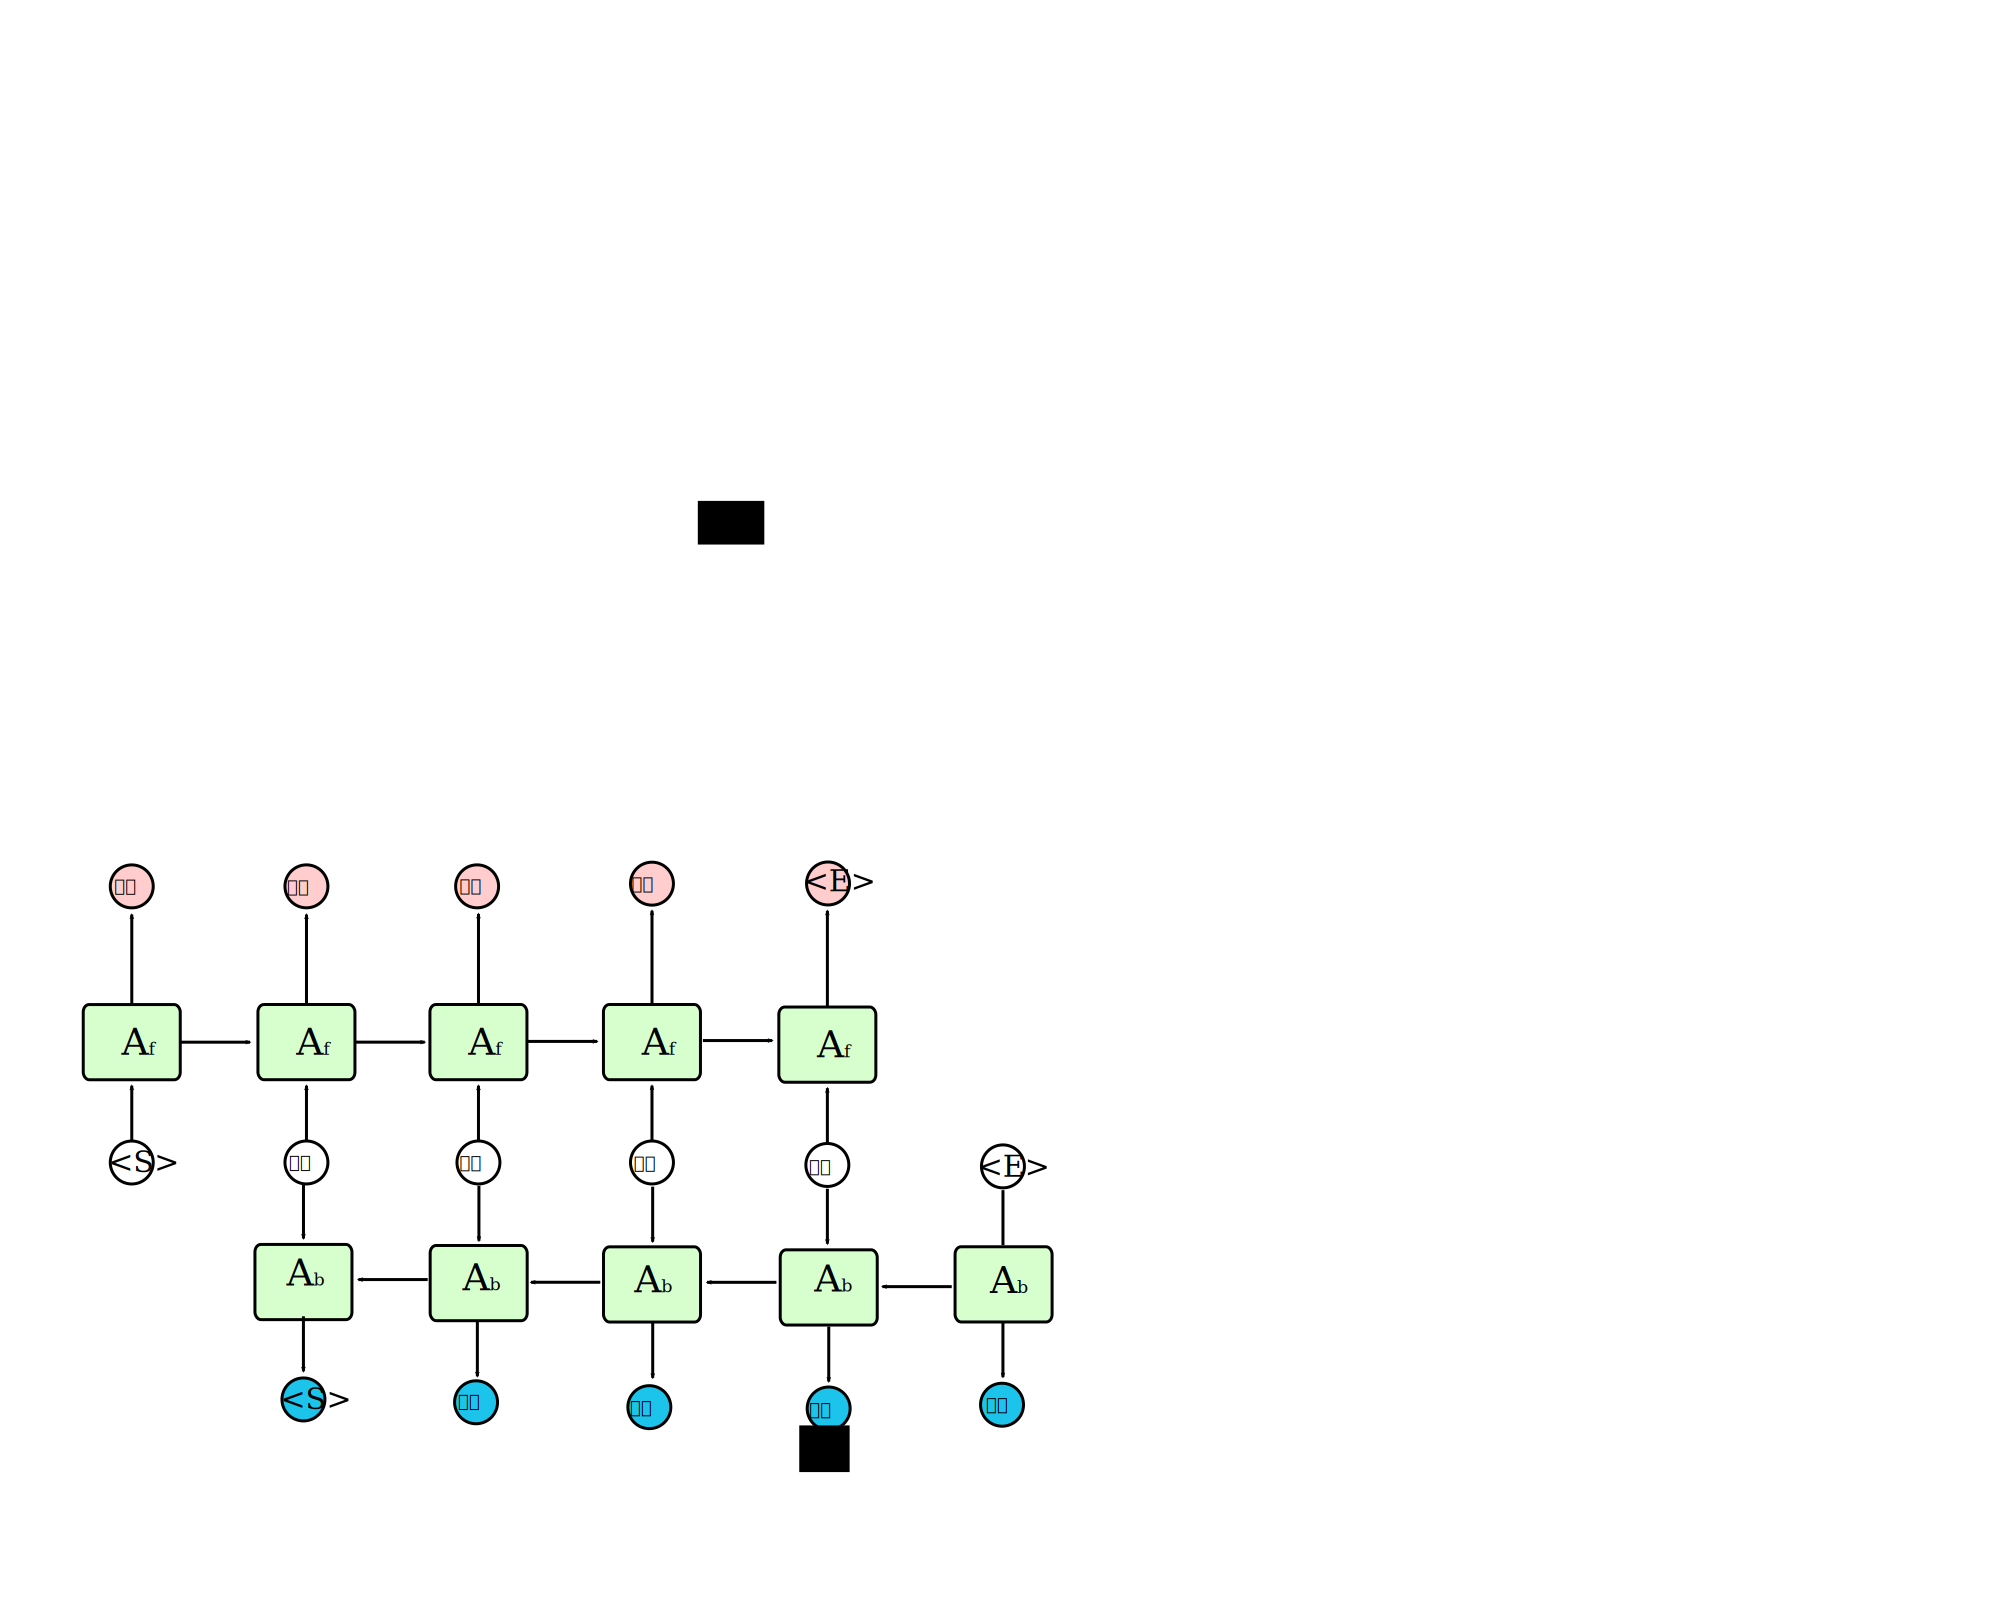
\includegraphics[width=3in,height=1.5in]{bilstm2.png}
        \caption{The Modified Bidirectional LSTM}
        \end{figure}
    \end{frame}

    \begin{frame}{Candidates Generation}
      \begin{itemize}
      \item Similar Posts
      \begin{equation}
         Score_{q,p}^1(q, p) = Sim_{LDA}(q, p) * Sim_{W2V}(q, p) * Sim_{LSTM}(q, p)
      \end{equation}
      \begin{equation}
         Score_{q,p}^2(q, p) = Sim_{LSA}(q, p) * Sim_{W2V}(q, p) * Sim_{LSTM}(q, p)
      \end{equation}
      \item Comment Candidates
      \begin{equation}
         Score_{q,c}^1(q, c) = Sim_{LSA}(q, c) * Sim_{W2V}(q, c)
      \end{equation}
      \begin{equation}
         Score_{q,c}^2(q, c) = Sim_{LDA}(q, c) * Sim_{W2V}(q, c)
      \end{equation}
    \end{itemize}
    \end{frame}

    \begin{frame}{Ranking}
      \begin{itemize}
        \item TextRank
        \item Pattern-IDF
        \item TextRank + Pattern-IDF
      \end{itemize}
    \end{frame}

    \begin{frame}{TextRank}
    \end{frame}

    \begin{frame}{Ranking}
      Inspired by PageRank. \newline

      For $N$ candidates, we construct $ N \times N $ matrix C. $C_{ij} = sim(candidate_i, candidate_j)$. Then we compute iteratively
      \[
      R(t+1) = 
      \begin{bmatrix}
          (1-d)/N       \\
          (1-d)/N       \\
          \hdotsfor{1} \\
          (1-d)/N       
      \end{bmatrix}
      +d
      \begin{bmatrix}
          C_{11} & C_{12} & C_{13} & \dots  & C_{1N} \\
          C_{21} & C_{22} & C_{23} & \dots  & C_{2N} \\
          \vdots & \vdots & \vdots & \ddots & \vdots \\
          C_{N1} & C_{N2} & C_{N3} & \dots  & C_{NN}
      \end{bmatrix}
      R(t)
      \]
      $R(0) = [1/N \ 1/N \ ... \ 1/N]^T$ \newline
      Stop when $|R(t+1)-R(t)|<\epsilon$
    \end{frame}

  \begin{frame}[standout]
    Questions?
  \end{frame}

\end{document}

